%!TeX root = ../main.tex

\section{Materiales y Metodolog\'ia}
En este trabajo se realizará el análisis de un motor de DC basándose en 
el esquema de la figura \ref{fig:MotorScheme}.
\begin{figure*}[t]
  \begin{center}
    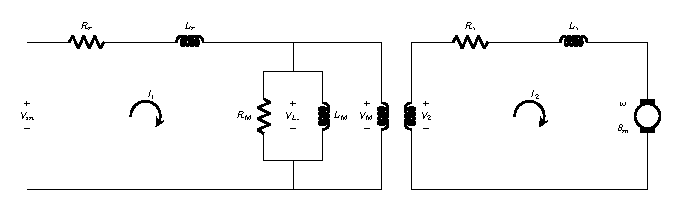
\includegraphics[width=0.98\linewidth]{img.tex-svg/MotorScheme.pdf}
    \caption{Esquema del motor de DC a analizar.}
    \label{fig:MotorScheme}
  \end{center}
\end{figure*}
Póstumo del cual se realizará una simulación en scilab con el fin de
corroborar los resultados y observar el comportamiento del motor
en el tiempo.

% Tex root = ../main.tex

\subsection{Modelado del motor en el espacio de estados}
El primer paso en el modelado del motor es analizar el comportamiento de
los componentes de interés. En este caso se considerará como entrada el
voltaje de entrada del motor ($V_{in}$), y como salida la velocidad
angular de la flecha ($\omega_m$).
Las variables de estado serán la corriente del sistema ($I_t$),
la posición angular ($\theta$) y la velocidad angular ($\omega_m$).
Tal como se muestra en la figura \ref{fig:Motor-LTI-CajaNegra}.
\begin{figure}[H]
  \begin{center}
    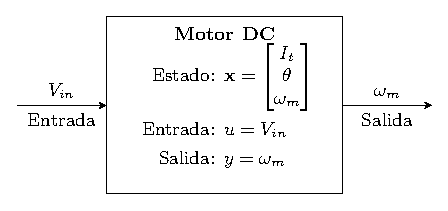
\includegraphics[width=0.98\linewidth]{img.tex-svg/Motor-LTI-CajaNegra.pdf}
    \caption{Esquema de caja negra con las variables de entrada, estado
    y salida del sistema modelado.}
    \label{fig:Motor-LTI-CajaNegra}
  \end{center}
\end{figure}

El modelo en espacio de estados se, tal como se muestra en el sistema
de ecuaciones \eqref{eq:EspacioEstados}.
\begin{equation}
  \label{eq:EspacioEstados}
  \begin{cases}
    \dot{\mathbf{x}} &= \mathbf{A} \mathbf{x} + \mathbf{B} u \\
    y &= \mathbf{C} \mathbf{x} + \mathbf{D} u
  \end{cases}
\end{equation}

\subsubsection{Análisis del voltaje en el rotor}

Para el análisis del sistema, se consideraron los voltajes para realizar
el modelado.

\begin{equation}
  \label{eq:Motor-LTI-Modelo}
  \begin{cases}
    V_r    &= iR  \\
    V_{L_r}&=L \frac{di}{dt}
  \end{cases}
\end{equation}

Donde i, representa a la corriente total del sistema.

También existe un voltaje negativo que se opone al voltaje de entrada:
la fuerza contraelectromotriz $V_M$, que se obtiene como efecto del proceso
electromagnético que ocurre dentro del motor.

Esta fuerza se vincula directamente con la velocidad angular de la flecha

$$V_{M} = K_e \omega_m$$

donde $K_e$ es la constante electromotriz.

Teniendo en cuenta estos elementos, es posible realizar el análisis de voltajes
en el rotor de un motor de DC.

\begin{equation*}
  \begin{cases}
    V_r    &= iR  \\
    V_{L_r}&=L \frac{di}{dt} \\
    V_{M}  &= K_e \omega_m
  \end{cases}
\end{equation*}
Y debido a que
$$
\sum_i V_i = 0
$$
Tenemos que los voltajes se relacionan de la forma
\begin{equation}
  \begin{aligned}
    -V_{in} + V_r + V_{L_r}       + V_{M} &= 0\\
    -V_{in} + Ri  + L\frac{di}{dt} + K_e\omega_m &= 0
  \end{aligned}
\end{equation}

De esta ecuación nos interesa el comportamiento de la corriente en el tiempo.
\begin{equation*}
  \begin{aligned}
    \frac1L \left(
      -V_{in} + Ri  + L\frac{di}{dt} + K_e\omega_m
    \right) &=\frac1L  (0) \\
      -\frac{V_{in}}L + \frac{Ri}L  + \frac{di}{dt} + \frac{K_e\omega_m}{L}
     &=  0 \\
  \end{aligned}
\end{equation*}
Obteniendo la siguiente ecuación diferencial
\begin{equation}
      \frac{di}{dt} = \frac{V_{in}}L - \frac{Ri}L  - \frac{K_e\omega_m}{L}
      \label{eq:DiferencialCorriente}
\end{equation}

Nuestras funciones en el espacio de estados se describen a partir de la
matriz

\subsubsection{Análisis mecánico del motor}
Al ser este tipo de sistemas un transformador (eléctrico-mecánico), se
necesita también conocer el comportamiento de la sección mecánica.

El par motriz $\tau_m$ es directamente proporcional al toque $K_t$ y la corriente
total de sistema $i$. El par de fricción viscoso $\tau_f$ es proporcional a
la velocidad angular $\omega_m$ y el coeficiente de fricción viscoso $B$.

\begin{equation*}
  \begin{cases}
    \tau_m = K_t i\\
    \tau_f = B \omega_m
  \end{cases}
\end{equation*}

De este modo, podemos a partir el esfuerzo de aceleración del motor $J$
podemos obtener la ecuación diferencial de la velocidad angular
\eqref{eq:DiferencialVelocidadAngular}.

\begin{equation*}
  \begin{aligned}
    J\frac{d\omega_m}{dt} &= \tau_m - \tau_f\\
   \frac1J  \left(
      J\frac{d\omega_m}{dt}
    \right)
   &=
   \frac1J  \left(
      \tau_m - \tau_f
    \right)\\
  \end{aligned}
\end{equation*}

\begin{equation}
  \frac{d\omega_m}{dt} = \frac{K_t i - B \omega_m}{J}\\
  \label{eq:DiferencialVelocidadAngular}
\end{equation}


\subsubsection{Matrices del sistema en el espacio de estados}
Es apreciable que las ecuaciones \eqref{eq:DiferencialCorriente} y
\eqref{eq:DiferencialVelocidadAngular} se puede obtener el
vector de ecuaciones diferenciales
$\dot{\mathbf{x}}$ de la forma

\begin{equation}
  \begin{cases}
    \dot{\mathbf{x}}&=\begin{bmatrix}
     -\frac{R}{L}   & 0 & -\frac{K_e}{L} \\
      0             & 0 &   1            \\
      \frac{K_t}{J} & 0 & -\frac{B}{J}   \\
    \end{bmatrix}
    \begin{bmatrix}
      I_t\\ \theta\\ \omega_m
    \end{bmatrix}
    +\begin{bmatrix} 
      \frac{1}{L} \\
      0\\
      0\\
    \end{bmatrix} u\\
    y &= \begin{bmatrix}
      0 & 0 & 1\\
    \end{bmatrix}
    \begin{bmatrix}
      I_t\\ \theta\\ \omega_m
    \end{bmatrix}
  \end{cases}
\end{equation}

De aquí es evidente que la posición angular no tiene efecto sobre
nuestra salida que es la velocidad angular.
Las matrices que obtenemos después del análisis se pueden apreciar
en la ecuación \eqref{eq:MatricesEspacioEstados}

\begin{equation}
  \begin{aligned}
    \mathbf{A} &= \begin{bmatrix}
    -\frac{R}{L}  & 0 & -\frac{K_e}{L} \\
    0             & 0 &  1           \\
    \frac{K_t}{J} & 0 & -\frac{B}{J} \\
  \end{bmatrix} &
    \mathbf{B} &= \begin{bmatrix}
    \frac{1}{L} \\
    0\\
    0\\
  \end{bmatrix} \\
  \mathbf{C} &= \begin{bmatrix}
      0 & 0 & 1
    \end{bmatrix} &
    \mathbf{D} &= 0
 \end{aligned}
  \label{eq:MatricesEspacioEstados}
\end{equation}

%! TeX root = ../main.tex

\subsection{Función de transferencia del sistema}
La función de transferencia $G(s)$ del sistema en el espacio de estados
se define de la forma

\begin{equation}
  G(s) = C(sI-A)^{-1}B + D
\end{equation}
 
\subsubsection{Desglose de $(sI-A)^{-1}$}

\begin{equation}
  \begin{aligned}
    sI-A &= \begin{bmatrix}
      s & 0 & 0 \\
      0 & s & 0 \\
      0 & 0 & s \\
    \end{bmatrix}
    - \begin{bmatrix}
      -\frac{R}{L}  & 0 &  -\frac{K_e}{L} \\
      0             & 0 &   1             \\
      \frac{K_t}{J} & 0 &  -\frac{B}{J}   \\
    \end{bmatrix}\\
    &= \begin{bmatrix}
      s+\frac{R}{L}    & 0-0 & 0+\frac{K_e}{L} \\
      0-0              & s-0 & 0-1             \\
      0-\frac{K_t}{J}  & 0-0 & s+\frac{B}{J}   \\
    \end{bmatrix}\\
    &= \begin{bmatrix}
      s+\frac{R}{L}  & 0 &  \frac{K_e}{L} \\
      0              & s & -1             \\
     -\frac{K_t}{J}  & 0 &  s+\frac{B}{J} \\
    \end{bmatrix}
  \end{aligned}
\end{equation}

Sabemos que la inversa de una matriz se define como en la ecuación \eqref{eq:InversaMatriz}

\begin{equation}
  Q^{-1} = \frac{1}{adj(Q)} Q^T
  \label{eq:InversaMatriz}
\end{equation}

Por lo tanto $(sI-A)^{-1} = \frac{1}{det(sI-A)}(sI-A)^T$ 

\begin{equation*}
  \begin{aligned}
    det(sI-A) &=
    \left(s+\frac{R}{L}\right)
    \begin{vmatrix}
      s & -1             \\
      0 &  s+\frac{B}{J} \\
    \end{vmatrix}\\
              &-
    0
    \begin{vmatrix}
      0             & -1             \\
      \frac{K_t}{J} &  s+\frac{B}{J} \\
    \end{vmatrix}
              +
    \frac{K_e}{L}
    \begin{vmatrix}
      0              & s  \\
     -\frac{K_t}{J}  & 0  \\
    \end{vmatrix}\\
    det(sI-A) &=
    \left(s+\frac{R}{L}\right)\left(s^2+\frac{B}{J}s\right) + 0 \\
    &+\frac{K_e}{L} \left(\frac{K_t}{J}s\right)\\
    det(sI-A) &=
    s^3 + \frac{B}{J}s^2 + \frac{R}{L}s^2 +\\ &+\frac{RB}{JL}s + \frac{K_t K_e}{JL}s\\
  \end{aligned}
\end{equation*}

\begin{equation}
  \begin{aligned}
    &det(sI-A) =\\
    &s^3 + \left(\frac{B}{J} + \frac{R}{L}\right)s^2 
    + \left(\frac{RB + K_t K_e}{JL}\right)s\\
  \end{aligned}
\end{equation}

\begin{equation*}
  \begin{aligned}
    &cof(sI-A) =\\ &\begin{bmatrix}
%%%%%%%%%TOP
      (-1)^{1+1}
      \begin{vmatrix}
        s             & -1              \\
        0             &  s+\frac{B}{J}  \\
      \end{vmatrix}&
      (-1)^{1+2}
      \begin{vmatrix}
        0             & -1              \\
       -\frac{K_t}{J} &  s+\frac{B}{J}  \\
      \end{vmatrix}&
      (-1)^{1+3}
      \begin{vmatrix}
        0             & s               \\
       -\frac{K_t}{J} & 0               \\
      \end{vmatrix}\\
%%%%%%%%MID
      (-1)^{2+1}
      \begin{vmatrix}
        0             &  \frac{K_e}{L} \\
        0             &  s+\frac{B}{J} \\
      \end{vmatrix}&
      (-1)^{2+2}
      \begin{vmatrix}
        s+\frac{R}{L} &  \frac{K_e}{L} \\
       -\frac{K_t}{J} &  s+\frac{B}{J} \\
      \end{vmatrix}&
      (-1)^{2+3}
      \begin{vmatrix}
        s+\frac{R}{L} & 0              \\
       -\frac{K_t}{J} & 0              \\
      \end{vmatrix}\\
%%%%%%%%BTM
      (-1)^{3+1}
      \begin{vmatrix}
        0 &  \frac{K_e}{L}             \\
        s & -1                         \\
      \end{vmatrix}&
      (-1)^{3+2}
      \begin{vmatrix}
        s+\frac{R}{L} &  \frac{K_e}{L} \\
        0             & -1             \\
      \end{vmatrix}&
      (-1)^{3+3}
      \begin{vmatrix}
        s+\frac{R}{L} & 0              \\
        0             & s              \\
      \end{vmatrix}\\
    \end{bmatrix}\\
  \end{aligned}
\end{equation*}

\begin{equation}
  \begin{aligned}
    &cof(sI-A) =\\
    &\begin{bmatrix}
      s^2 + \frac{B}{J}s  &  \frac{K_t}{J}                                                  &  \frac{K_t}Js   \\
      0                   &  s^2 + \left(\frac{R}L + \frac{B}J\right)s + \frac{K_e K_t}{JL} &  0              \\
      -\frac{K_e}L s      &  s +\frac{R}L                                                   &  s^2+\frac{R}Ls \\
    \end{bmatrix}
  \end{aligned}
\end{equation}

\begin{equation}
  \begin{aligned}
    &adj(sI-A) =\\
    &\begin{bmatrix}
      s^2 + \frac{B}{J}s                                             &   
      0                                                              &   
     -\frac{K_e}L s                                                  \\  
      \frac{K_t}{J}                                                  & 
      s^2 + \left(\frac{R}L + \frac{B}J\right)s + \frac{K_e K_t}{JL} & 
      s +\frac{R}L                                                   \\
      \frac{K_t}Js                                                   &
      0                                                              &
      s^2+\frac{R}Ls                                                   \\
    \end{bmatrix}
  \end{aligned}
\end{equation}

\subsubsection{Función de transferencia del sistema}

\begin{equation*}
  q(s) = s^2 + \left(\frac{R}L + \frac{B}J\right)s + \frac{K_e K_t}{JL}
\end{equation*}

\begin{multline*}
  G(s) =
    \frac{1}{s^3 + \left(\frac{B}{J} + \frac{R}{L}\right)s^2 + \left(\frac{RB + K_t K_e}{JL}\right)s}\\
    \begin{bmatrix}
      0 & 0 & 1 \\
    \end{bmatrix}
    \begin{bmatrix}
      s^2 + \frac{B}{J}s  &   
      0                   &   
     -\frac{K_e}L s       \\  
      \frac{K_t}{J}       & 
      q(s)                & 
      s +\frac{R}L        \\
      \frac{K_t}Js        &
      0                   &
      s^2+\frac{R}Ls      \\
    \end{bmatrix}
    \begin{bmatrix}
      \frac1L \\ 0 \\ 0 \\
    \end{bmatrix}
\end{multline*}

\begin{multline*}
  G(s) =
    \frac{1}{s^3 + \left(\frac{B}{J} + \frac{R}{L}\right)s^2 + \left(\frac{RB + K_t K_e}{JL}\right)s}\\
    \frac1L
    \begin{bmatrix}
      0 & 0 & 1 \\
    \end{bmatrix}
    \begin{bmatrix}
      s^2 + \frac{B}{J}s  \\
      \frac{K_t}{J}       \\
      \frac{K_t}Js        \\
    \end{bmatrix}
\end{multline*}

\begin{equation}
  G(s) =
    \frac{\frac{K_t}{JL}s}{s^3 + \left(\frac{B}{J} + \frac{R}{L}\right)s^2 + \left(\frac{RB + K_t K_e}{JL}\right)s}
\end{equation}


\subsubsection{Función de transferencia con valores experimentales}

A partir de los mismos valores experimentales: $R = 2.1\ \Omega$, $L = 5\times10^{-3}\ \text{H}$, $K_t = 0.12\ \text{N·m/A}$, $K_e = 0.12\ \text{V/(rad/s)}$, $J = 1\times10^{-4}\ \text{kg·m}^2$ y $B = 1\times10^{-5}\ \text{N·m·s/rad}$, la función de transferencia numérica resulta:

\begin{equation*}
  \begin{aligned}
    &G(s) =\\
    &\frac{\tfrac{0.12}{1\mathrm{e}{-4} \cdot 5\mathrm{e}{-3}}s}{s^{3} + \left(\tfrac{1\mathrm{e}{-5}}{1\mathrm{e}{-4}} + \tfrac{2.1}{5\mathrm{e}{-3}}\right)s^{2} + \left(\tfrac{2.1\cdot1\mathrm{e}{-5} + 0.12\cdot0.12}{1\mathrm{e}{-4} \cdot 5\mathrm{e}{-3}}\right)s}\\
    &G(s) =
    \frac{2.4\mathrm{e}^{5}\,s}{s^{3} + 4.201\mathrm{e}^{2}\,s^{2} + 2.8842\mathrm{e}^{4}\,s} 
  \end{aligned}
\end{equation*}

\begin{equation}
G(s) = \frac{2.4\mathrm{e}^{5}}{s^{2} + 4.201\mathrm{e}^{2}\,s + 2.8842\mathrm{e}^{4}}
\label{eq:TransferFunctionNumeric}
\end{equation}

%!TeX root = ../main.tex

\subsection{Análisis de estabilidad del sistema}

El análisis de estabilidad del sistema se realiza utilizando la matriz
dinámica $\mathbf{A}$ y a través de la definición de Lyapunov.

%!TeX root = ../main.tex

\subsection{Análisis de estabilidad del sistema a través de la matriz dinámica}
Para este análisis se realizará un determinante y la
obtención de los autovalores con el fin de conocer los puntos de estabilidad
del sistema.

\subsubsection{Determinante de $\mathbf{A}$}

\begin{align*}
  det\left(\mathbf{A}\right) &=
  det\begin{bmatrix}
  -\frac{R}{L}          & 0        & -\frac{K_e}{L}   \\
  0                     & 0        &  1               \\
  \frac{K_t}{J}         & 0        & -\frac{B}{J}     \\
  \end{bmatrix} \\
\end{align*}
\begin{align*}
  %%% det(A)
  &det\left(\mathbf{A}\right) =\\
%  \left(-\tfrac{R}{L} \right)
%  \begin{vmatrix}
%    0              &  1           \\
%    0              & -\frac{B}{J} \\
%  \end{vmatrix}
%  -\left(0\right)
%  \begin{vmatrix}
%    0              &  1           \\
%    \frac{K_t}{J}  & -\frac{B}{J} \\
%  \end{vmatrix}
%  +\left(-\tfrac{K_e}{L}\right)
%  \begin{vmatrix}
%    0              & 0            \\
%    \frac{K_t}{J}  & 0            \\
%  \end{vmatrix}\\
  &\begin{bmatrix}
    -\tfrac{R}{L} 
    -0
    +-\tfrac{K_e}{L}
  \end{bmatrix}
  \begin{bmatrix}
    \begin{vmatrix}
      0              &  1           \\
      0              & -\frac{B}{J} \\
    \end{vmatrix}\\
    \begin{vmatrix}
      0              &  1           \\
      \frac{K_t}{J}  & -\frac{B}{J} \\
    \end{vmatrix}\\
    \begin{vmatrix}
      0              & 0            \\
      \frac{K_t}{J}  & 0            \\
    \end{vmatrix}
  \end{bmatrix}\\
  %%% det(A)
  %%% det(A)
  &det\left(\mathbf{A}\right) = 0
\end{align*}

Dicho determinante implica que el sistema tiene infinitos puntos
de estabilidad.

\subsubsection{Autovalores de $\mathbf{A}$}
Los autovalores son aquellos valores $\lambda$ que cumplen con
la ecuación \eqref{eq:DefinicionAutovalores}.
\begin{equation}
  det\left(\mathbf{A-\lambda I}\right)=0
  \label{eq:DefinicionAutovalores}
\end{equation}

Por lo tanto se necesita obtener la matriz \eqref{eq:Matriz A - lambda I}.

\begin{equation}
  \mathbf{A-\lambda I} =
  \begin{bmatrix}
  -\frac{R}{L}          & 0        & -\frac{K_e}{L}   \\
  0                     & 0        &  1               \\
  \frac{K_t}{J}         & 0        & -\frac{B}{J}     \\
  \end{bmatrix}
  \label{eq:Matriz A - lambda I}
\end{equation}

luego, se obtiene el determinante de \eqref{eq:Matriz A - lambda I}
que resulta ser un polinomio de tercer grado \eqref{eq:detA - lI}

\begin{align*}
  det\left(\mathbf{A-\lambda I}\right) &=
  det\begin{bmatrix}
  -\frac{R}{L}-\lambda  & 0        & -\frac{K_e}{L}         \\
  0                     & -\lambda &  1                     \\
  \frac{K_t}{J}         & 0        & -\frac{B}{J} - \lambda \\
  \end{bmatrix} \\
  %%% det(A)
  det\left(\mathbf{A-\lambda I}\right) &=
  \left(-\tfrac{R}{L} - \lambda\right)
  \begin{vmatrix}
    -\lambda       &  1                     \\
    0              & -\frac{B}{J} - \lambda \\
  \end{vmatrix}\\
  &-\left(0\right)
  \begin{vmatrix}
    0              &  1                     \\
    \frac{K_t}{J}  & -\frac{B}{J} - \lambda \\
  \end{vmatrix}\\
  &+\left(-\tfrac{K_e}{L}\right)
  \begin{vmatrix}
    0              & -\lambda               \\
    \frac{K_t}{J}  & 0                      \\
  \end{vmatrix}
\end{align*}

\begin{equation}
  \begin{aligned}
    %%% det(A)
    &det\left(\mathbf{A-\lambda I}\right) = \\
    &\left(-\tfrac{R}{L}-\lambda\right)\left(\tfrac{B}{J}\lambda+\lambda^2\right)
    -\left(\tfrac{K_e K_t}{JL}\lambda\right)
    \label{eq:detA  - lI}
  \end{aligned}
\end{equation}

Luego de obtener \eqref{eq:detA  - lI}, a fin de rescatar los autovalores se procede
a resolver la expresión \eqref{eq:DefinicionAutovalores} para la matriz \eqref{eq:Matriz A - lambda I}

\begin{equation*}
  \begin{aligned}
    det\left(\mathbf{A-\lambda I}\right) &=0  \\
    \left(-\tfrac{R}{L}-\lambda\right)\left(\tfrac{B}{J}\lambda+\lambda^2\right)
    -\left(\tfrac{K_e K_t}{JL}\lambda\right)
                                         &=0  \\
    \lambda\left[
    \left(-\tfrac{R}{L}-\lambda\right)\left(\tfrac{B}{J}+\lambda\right)
    -\tfrac{K_e K_t}{JL}
    \right]
                                         &=0  \\
    -\lambda\left[
    \left(\tfrac{R}{L}+\lambda\right)\left(\tfrac{B}{J}+\lambda\right)
    +\tfrac{K_e K_t}{JL}
    \right]
                                         &=0  \\
  \end{aligned}
\end{equation*}

La primera solución se puede encontrar de la forma mostrada en \eqref{eq:SolucionAutovalores 1}

Definiendo $p= \left(\tfrac{R}{L}+\lambda\right)\left(\tfrac{B}{J}+\lambda\right)
    +\tfrac{K_e K_t}{JL} $
\begin{equation}
  \begin{aligned}
    \frac1{-p}\left(-\lambda p\right)
     &=\frac1{-p}0\\
    \lambda_1 &=0\\
     \label{eq:SolucionAutovalores 1}
  \end{aligned}
\end{equation}

De manera análoga es posible encontrar los segundo y tercer autovalores
obteniendo la igualdad respecto a $p$ y resolviendo la ecuación
de segundo grado \eqref{eq:SolucionAutovalores 2} que se obtiene,
resultando en la expresión \eqref{eq:SolucionAutovalores 3}.

\begin{equation*}
  \begin{aligned}
    \frac1{-\lambda}\left(-\lambda p\right)
     &=\frac1{-\lambda}0\\
    p &=0\\
  \end{aligned}
\end{equation*}

\begin{equation}
  \begin{aligned}
    \left(\tfrac{R}{L}+\lambda\right)\left(\tfrac{B}{J}+\lambda\right)
    +\tfrac{K_e K_t}{JL} &=0
     \label{eq:SolucionAutovalores 2}
  \end{aligned}
\end{equation}

\begin{equation*}
      \lambda^2 + \left(\tfrac{B}{J} + \tfrac{R}{L}\right)\lambda
    +\tfrac{BR+K_e K_t}{JL} =0
\end{equation*}
\begin{equation}
  \begin{aligned}
    &\lambda_{2,3} = \\
    &\frac{
      - \left( \tfrac{B}{J} + \tfrac{R}{L} \right)
      \pm \sqrt{
        \left( \tfrac{B}{J} + \tfrac{R}{L} \right)^2
        - 4 \tfrac{BR+K_e K_t}{JL}
      }
    }
    {2}
  \end{aligned}
     \label{eq:SolucionAutovalores 3}
\end{equation}

\subsubsection{Análisis de autovalores con valores experimentales}

A partir de valores experimentales indicados en \cite{Ugurlu2025} para un motor de DC, se obtienen autovalores numéricos que ilustran la dinámica del sistema. Los parámetros utilizados como ejemplo son: resistencia $R = 2.1\ \Omega$, inductancia $L = 5\times10^{-3}\ \text{H}$, constante de par $K_t = 0.12\ \text{N·m/A}$, constante de fuerza contraelectromotriz $K_e = 0.12\ \text{V/(rad/s)}$, momento de inercia $J = 1\times10^{-4}\ \text{kg·m}^2$ y coeficiente de fricción viscosa $B = 1\times10^{-5}\ \text{N·m·s/rad}$.

Sustituyendo estos valores en la expresión general para $\lambda_{2,3}$ de \eqref{eq:SolucionAutovalores 3}, y definiendo  
\[
\delta = \left(\tfrac{B}{J} + \tfrac{R}{L}\right)^2 - 4 \tfrac{BR+K_e K_t}{JL},
\]  
se calcula:

\begin{equation*}
\begin{aligned}
\tfrac{B}{J} + \tfrac{R}{L} &= \tfrac{1\mathrm{e}{-5}}{1\mathrm{e}{-4}} + \tfrac{2.1}{5\mathrm{e}{-3}} \\
&= 1\mathrm{e}{-1} + 4.2\mathrm{e}{2} = 4.201\mathrm{e}{2} \\[2pt]
\left(\tfrac{B}{J} + \tfrac{R}{L}\right)^2 &= (4.201\mathrm{e}{2})^{2} = 1.76484\mathrm{e}{5} \\[2pt]
4 \tfrac{BR+K_e K_t}{JL} &= 4 \cdot \tfrac{(2.1\mathrm{e}{0})(1\mathrm{e}{-5}) + (1.2\mathrm{e}{-1})(1.2\mathrm{e}{-1})}{(1\mathrm{e}{-4})(5\mathrm{e}{-3})} \\
&= 4 \cdot \tfrac{2.1\mathrm{e}{-5} + 1.44\mathrm{e}{-2}}{5\mathrm{e}{-7}} \\
&= 4 \cdot \tfrac{1.4421\mathrm{e}{-2}}{5\mathrm{e}{-7}} \\
&= 4 \cdot 2.8842\mathrm{e}{4} = 1.15368\mathrm{e}{5} \\[2pt]
\delta &= 1.76484\mathrm{e}{5} - 1.15368\mathrm{e}{5}\\
       &= 6.1116\mathrm{e}{4} \\[2pt]
\sqrt{\delta} &\approx 2.4722\mathrm{e}{2}
\end{aligned}
\end{equation*}
Luego, los autovalores no nulos resultan:

\begin{equation*}
\begin{aligned}
\lambda_{2,3} &= \frac{ - \left( \tfrac{B}{J} + \tfrac{R}{L} \right) \pm \sqrt{\delta}}{2} \\[2pt]
\lambda_2 &\approx \frac{-4.201\mathrm{e}{2} + 2.4722\mathrm{e}{2}}{2} \approx  86.44 \\[2pt]
\lambda_3 &\approx \frac{-4.201\mathrm{e}{2} - 2.4722\mathrm{e}{2}}{2} \approx -333.66
\end{aligned}
\end{equation*}

De este modo, el conjunto completo de autovalores para este caso de ejemplo es:
\begin{equation}
    \lambda_1 = 0,\quad \lambda_2 \approx -86.44,\quad \lambda_3 \approx -333.66
    \label{eq:ResultadoAutovaloresExperimental}
\end{equation}

\subsubsection{Conclusión del análisis de estabilidad por medio de la matriz dinámica}

Debido a que la matriz dinámica tiene un autovalor $\lambda={0}$, se puede
concluir que el sistema es marginalmente estable.

%!TeX root = ../main.tex

\subsection{Análisis de estabilidad del sistema a través del criterio de Lyapunov}

El criterio de Lyapunov implica la existencia de una función $\mathbf{V}(x)$ considerada
función candidata, dicha función definida en \eqref{eq:DefiniciónLyapunovV} requiere de
una matriz $P$ que sea positiva definida.
Dicha función $\mathbf{V}(x)$ deberá ser definida positiva y su derivada temporal
$\mathbf{\dot{V}}(x)$ deberá definida negativa o semidefinida negativa.

\begin{equation}
  \begin{aligned}
    \mathbf{V}(x)       &= \mathbf{x}^TP\mathbf{x},\qquad P=P^T > 0  \\
    \mathbf{\dot{V}}(x) &= \mathbf{x}^T \left(\mathbf{A} P + P \mathbf{A} \right)\mathbf{x}
    \label{eq:DefiniciónLyapunovV}
  \end{aligned}
\end{equation}

\subsubsection{Función candidata de Lyapunov}

Para simplificar el análisis, se considera una matriz $P$ diagonal con elementos
positivos \eqref{eq:PDiagonal}.

\begin{equation}
    P = \begin{bmatrix}
        \alpha & 0 & 0 \\
        0 & \beta & 0 \\
        0 & 0 & \gamma
    \end{bmatrix}, \quad \alpha, \beta, \gamma > 0
    \label{eq:PDiagonal}
\end{equation}

\subsubsection{Desarrollo de la función candidata}
Sustituyendo la matriz diagonal $P$ de \eqref{eq:PDiagonal} y el vector de estado $\mathbf{x} = [i, \theta, \omega]^T$ en la definición general \eqref{eq:DefiniciónLyapunovV}, se obtiene la función candidata concreta.
\begin{equation*}
    \begin{aligned}
        \mathbf{V}(\mathbf{x}) &= \mathbf{x}^T P \mathbf{x}\\
        \mathbf{V}(\mathbf{x}) &=
        \begin{bmatrix}
            i & \theta & \omega
        \end{bmatrix}
        \begin{bmatrix}
            \alpha & 0 & 0 \\
            0 & \beta & 0 \\
            0 & 0 & \gamma
        \end{bmatrix}
        \begin{bmatrix}
            i \\ \theta \\ \omega
        \end{bmatrix}
    \end{aligned}
\end{equation*}
\begin{equation}
        \mathbf{V}(\mathbf{x}) =
        \alpha i^2 + \beta \theta^2 + \gamma \omega^2
        \label{eq:LyapunovCandidata}
\end{equation}

Sustituyendo la matriz $\mathbf{A}$ y la matriz $P$ diagonal en la expresión $\mathbf{A}^T P + P \mathbf{A}$ se obtiene la expresión \eqref{eq:ATPPA}.

\begin{equation}
    \mathbf{A}^T P + P \mathbf{A} = 
    \begin{bmatrix} 
        -2\frac{R}{L}\alpha & 0 & \frac{K_t}{J}\gamma - \frac{K_e}{L}\alpha \\
        0 & 0 & \beta \\
        \frac{K_t}{J}\gamma - \frac{K_e}{L}\alpha & \beta & -2\frac{B}{J}\gamma
    \end{bmatrix}
    \label{eq:ATPPA}
\end{equation}

\subsubsection{Condición para simplificar la matriz}

Para eliminar los términos cruzados (1,3) y (3,1) se impone la condición
\eqref{eq:CondicionCruzados}.

\begin{equation}
    \frac{K_t}{J}\gamma - \frac{K_e}{L}\alpha = 0
    \label{eq:CondicionCruzados}
\end{equation}

Asumiendo que $K_e = K_t$ en unidades consistentes\footnote{Esto se puede considerar
porque en un motor DC ideal, sin pérdidas, la potencia eléctrica que entra es igual
a la potencia mecánica que sale. Es decir, el voltaje contraelectromotriz por la
corriente es igual al par por la velocidad.}, se obtiene la relación
\eqref{eq:GammaAlpha}.

\begin{equation}
    \gamma = \frac{J}{L} \alpha
    \label{eq:GammaAlpha}
\end{equation}

Sustituyendo \eqref{eq:GammaAlpha} en \eqref{eq:ATPPA}, la matriz se simplifica
a \eqref{eq:ATPPASimplificada}.

\begin{equation}
    \mathbf{A}^T P + P \mathbf{A} = 
    \begin{bmatrix} 
        -2\frac{R}{L}\alpha & 0 & 0 \\
        0 & 0 & \beta \\
        0 & \beta & -2\frac{B}{L}\alpha
    \end{bmatrix}
    \label{eq:ATPPASimplificada}
\end{equation}

\subsubsection{Derivada de la función de Lyapunov}

La derivada temporal de la función de Lyapunov resulta en la expresión
\eqref{eq:DotVFinal}.

\begin{equation}
    \mathbf{\dot{V}}(\mathbf{x}) = -2\alpha\left( \frac{R}{L} i^2 + \frac{B}{L} \omega^2 \right) + 2\beta \theta \omega
    \label{eq:DotVFinal}
\end{equation}

\subsubsection{Verificación de las condiciones de Lyapunov}

La función $\mathbf{V}(\mathbf{x}) = \alpha i^2 + \beta \theta^2 + \gamma \omega^2$ es
definida positiva para $\alpha, \beta, \gamma > 0$. Sin embargo, la derivada
$\mathbf{\dot{V}}(\mathbf{x})$ no es definida negativa para todos los estados debido al
término $2\beta \theta \omega$. Si se considera $\beta = 0$, la derivada se
reduce a \eqref{eq:DotVSimplificada}.

\begin{equation}
    \mathbf{\dot{V}}(\mathbf{x}) = -2\alpha\left( \frac{R}{L} i^2 + \frac{B}{L} \omega^2 \right) \leq 0
    \label{eq:DotVSimplificada}
\end{equation}

La función candidata de Lyapunov en \eqref{eq:LyapunovCandidata} es definida positiva
y su derivada en \eqref{eq:DotVSimplificada} es semidefinida negativa, lo que
satisface las condiciones para estabilidad en el sentido de Lyapunov. Esta
estabilidad no es asintótica, pues $\mathbf{\dot{V}}(\mathbf{x})$ se anula para
$i=0$, $\omega=0$ y cualquier valor de $\theta$, lo cual refleja directamente
el autovalor en cero de la matriz dinámica $\mathbf{A}$.


%!TeX root = ../main.tex

\subsection{Análisis de controlabilidad del sistema}
La matriz de controlabilidad se define de la forma
\begin{equation}
  \mathcal{C} = \begin{bmatrix}
    \mathbf{B} & \mathbf{A}\mathbf{B} & \cdots & \mathbf{A}^{n-1}\mathbf{B}
  \end{bmatrix} 
\end{equation}

Nuestro sistema corresponde a un orden 3, por lo tanto, su matriz de controlabilidad
está dada por la expresión \eqref{eq:DefiniciónMatrizControlabilidadMotor}

\begin{equation}
  \mathcal{C} = \begin{bmatrix}
    \mathbf{B} & \mathbf{A}\mathbf{B} & \mathbf{A}^{2}\mathbf{B}
  \end{bmatrix} 
  \label{eq:DefiniciónMatrizControlabilidadMotor}
\end{equation}

\begin{equation*}
  \begin{aligned}
    \mathbf{AB} &= 
    \begin{bmatrix}
      -\frac{R}{L}  & 0 & -\frac{K_e}{L} \\
      0             & 0 &  1             \\
      \frac{K_t}{J} & 0 & -\frac{B}{J}   \\
    \end{bmatrix}
    \begin{bmatrix}
      \frac{1}{L} \\
      0           \\
      0           \\
    \end{bmatrix} \\
     &= 
    \begin{bmatrix}
      -\frac{R}{L^2}  \\
      0               \\
      \frac{K_t}{JL}  \\
    \end{bmatrix}
  \end{aligned}
\end{equation*}

\begin{equation*}
  \begin{aligned}
    &\mathbf{A^2B} =\\
    &\begin{bmatrix}
       \tfrac{R^2}{L^2} - \tfrac{K_e K_t}{JL}                 & 0 & \tfrac{K_e}{L}\left(\tfrac{B}{J} + \tfrac{R}{L}\right) \\
       \tfrac{K_t}{J}                                         & 0 & -\tfrac{B}{J}                                          \\
      -\tfrac{K_t}{J}\left(\tfrac{R}{L} + \tfrac{B}{J}\right) & 0 & \tfrac{B^2}{J^2} - \tfrac{K_e K_t}{JL}
    \end{bmatrix}
    \begin{bmatrix}
      \frac{1}{L} \\
      0\\
      0\\
    \end{bmatrix} \\
    &\mathbf{A^2B} =\\
    &\begin{bmatrix}
       \tfrac{R^2}{L^2} - \tfrac{K_e K_t}{JL}                 \\
       \tfrac{K_t}{J}                                         \\
      -\tfrac{K_t}{J}\left(\tfrac{R}{L} + \tfrac{B}{J}\right) \\
    \end{bmatrix}
  \end{aligned}
\end{equation*}

\begin{equation}
  \mathcal{C} = 
  \begin{bmatrix}
    \tfrac{1}{L}     & -\tfrac{R}{L^2}  & \tfrac{R^2}{L^3} - \tfrac{K_e K_t}{JL^2}                  \\
    0                & 0                & \tfrac{K_t}{JL}                                           \\
    0                & \tfrac{K_t}{JL}  & -\tfrac{K_t}{JL}\left( \tfrac{R}{L} + \tfrac{B}{J} \right)
  \end{bmatrix}
  \label{eq:MatrizControlabilidadMotor}
\end{equation}

\subsubsection{Reducción de la matriz de controlabilidad}

\begin{equation*}
  \mathcal{C} = 
  \begin{bmatrix}
      \frac{1}{L} &  -\frac{R}{L^2}   &  \frac{R^2}{L^3}-\frac{K_e K_t}{JL^2}  \\
      0           &   0               &  \frac{K_t}{JL}                        \\
      0           &   \frac{K_t}{JL}  &  -\frac{K_t}{JL}\left(\frac{R}{L}+\frac{B}{J}\right) \\
  \end{bmatrix}
\end{equation*}

\begin{equation*}
  \begin{aligned}
    &R_1\leftarrow L R_1\\
    &\mathcal{C} = 
    \begin{bmatrix}
      1           &  -\frac{R}{L}     &  \frac{R^2}{L^2}-\frac{K_e K_t}{JL}    \\
      0           &   0               &  \frac{K_t}{JL}                        \\
      0           &   \frac{K_t}{JL}  &  -\frac{K_t}{JL}\left(\frac{R}{L}+\frac{B}{J}\right) \\
    \end{bmatrix}
  \end{aligned}
\end{equation*}

\begin{equation*}
  \begin{aligned}
    &R_2 \leftrightarrow R_3 \quad \text{(intercambio de filas)}\\
    &\mathcal{C} = 
    \begin{bmatrix}
      1           &  -\frac{R}{L}     &  \frac{R^2}{L^2}-\frac{K_e K_t}{JL}    \\
      0           &   \frac{K_t}{JL}  &  -\frac{K_t}{JL}\left(\frac{R}{L}+\frac{B}{J}\right) \\
      0           &   0               &  \frac{K_t}{JL}                        \\
    \end{bmatrix}
  \end{aligned}
\end{equation*}

\begin{equation*}
  \begin{aligned}
    &R_2 \leftarrow \tfrac{JL}{K_t} R_2\\
    &\mathcal{C} = 
    \begin{bmatrix}
      1           &  -\frac{R}{L}     &  \frac{R^2}{L^2}-\frac{K_e K_t}{JL}    \\
      0           &   1               &  -\left(\frac{R}{L}+\frac{B}{J}\right) \\
      0           &   0               &  \frac{K_t}{JL}                        \\
    \end{bmatrix}
  \end{aligned}
\end{equation*}

\begin{equation*}
  \begin{aligned}
    &R_3 \leftarrow \tfrac{JL}{K_t} R_3\\
    &\mathcal{C} = 
    \begin{bmatrix}
      1           &  -\frac{R}{L}     &  \frac{R^2}{L^2}-\frac{K_e K_t}{JL}    \\
      0           &   1               &  -\left(\frac{R}{L}+\frac{B}{J}\right) \\
      0           &   0               &  1                                     \\
    \end{bmatrix}
  \end{aligned}
\end{equation*}

\begin{equation*}
  \begin{aligned}
    &R_2 \leftarrow R_2 + \left(\frac{R}{L}+\frac{B}{J}\right) R_3\\
    &\mathcal{C} = 
    \begin{bmatrix}
      1           &  -\frac{R}{L}     &  \frac{R^2}{L^2}-\frac{K_e K_t}{JL}    \\
      0           &   1               &  0                                     \\
      0           &   0               &  1                                     \\
    \end{bmatrix}
  \end{aligned}
\end{equation*}

\begin{equation*}
  \begin{aligned}
    &R_1 \leftarrow R_1 + \tfrac{R}{L} R_2\\
    &\mathcal{C} = 
    \begin{bmatrix}
      1           &   0               &  \frac{R^2}{L^2}-\frac{K_e K_t}{JL}    \\
      0           &   1               &  0                                     \\
      0           &   0               &  1                                     \\
    \end{bmatrix}
  \end{aligned}
\end{equation*}

\begin{equation*}
  \begin{aligned}
    &R_1 \leftarrow R_1 + \left(\tfrac{K_t K_e}{JL}-\tfrac{R^2}{L^2}\right) R_3\\
    &\mathcal{C} = 
    \begin{bmatrix}
      1           &   0               &  0                                     \\
      0           &   1               &  0                                     \\
      0           &   0               &  1                                     \\
    \end{bmatrix}
  \end{aligned}
\end{equation*}

Debido a que el rango de la matriz $\mathcal{C}$ es completo, se puede afirmar que el sistema es controlable.

\subsubsection{Matriz de controlabilidad con valores experimentales}

Con los parámetros experimentales: $R = 2.1\,\Omega$, $L = 0.005\,\text{H}$,
$K_t = 0.12\,\text{N·m/A}$, $K_e = 0.12\,\text{V/(rad/s)}$, $J = 0.0001\,\text{kg·m}^2$
y $B = 1\times10^{-5}\,\text{N·m·s/rad}$, la matriz de controlabilidad numérica es:

\begin{equation*}
  \begin{aligned}
    &\mathcal{C}_{\text{num}} = \\
    &\begin{bmatrix}
      \tfrac{1}{5\mathrm{e}{-3}} & -\tfrac{2.1}{(5\mathrm{e}{-3})^2} & \tfrac{(2.1)^2}{(5\mathrm{e}{-3})^3} - \tfrac{(0.12)^2}{1\mathrm{e}{-4} \cdot (5\mathrm{e}{-3})^2} \\[2pt]
      0 & 0 & \tfrac{0.12}{1\mathrm{e}{-4} \cdot 5\mathrm{e}{-3}} \\[2pt]
      0 & \tfrac{0.12}{1\mathrm{e}{-4} \cdot 5\mathrm{e}{-3}} & -\tfrac{0.12}{1\mathrm{e}{-4} \cdot 5\mathrm{e}{-3}}\left( \tfrac{2.1}{5\mathrm{e}{-3}} + \tfrac{1\mathrm{e}{-5}}{1\mathrm{e}{-4}} \right)
    \end{bmatrix}
  \end{aligned}
\end{equation*}

\begin{equation}
\mathcal{C}_{\text{num}} = 
\begin{bmatrix}
    2.0\mathrm{e}^{2} & -8.4\mathrm{e}^{4} & 2.95\mathrm{e}^{7} \\[2pt]
    0 & 0 & 2.4\mathrm{e}^{5} \\[2pt]
    0 & 2.4\mathrm{e}^{5} & -1.01\mathrm{e}^{8}
\end{bmatrix}
\label{eq:MatrizControlabilidadMotorValoresExperimentales}
\end{equation}

%! TeX root = ../main.tex

\subsection{Análisis de observabilidad del sistema}
La matriz de observabilidad de un sistema se define de la forma

\begin{equation}
  \mathcal{O} = \begin{bmatrix}
    \mathbf{C} \\ \mathbf{C}\mathbf{A} \\ \vdots \\ \mathbf{C}\mathbf{A}^{n-1}
  \end{bmatrix} 
\end{equation}

Debido a que el sistema corresponde al orden 3, su matriz de observabilidad
está dada por la expresión \eqref{eq:MatrizObservabilidad}

\begin{equation}
  \mathcal{O} = \begin{bmatrix}
    \mathbf{C} \\ \mathbf{C}\mathbf{A} \\ \mathbf{C}\mathbf{A}^{2}
  \end{bmatrix} 
  \label{eq:MatrizObservabilidad}
\end{equation}

\begin{equation*}
  \begin{aligned}
    \mathbf{CA} &= 
    \begin{bmatrix}
      0 &
      0 &
      1 \\
    \end{bmatrix}
    \begin{bmatrix}
      -\frac{R}{L}  & 0 & -\frac{K_e}{L} \\
      0             & 0 &  1             \\
      \frac{K_t}{J} & 0 & -\frac{B}{J}   \\
    \end{bmatrix} \\
     &= 
    \begin{bmatrix}
      \frac{K_t}{J} & 0 & -\frac{B}{J}   \\
    \end{bmatrix}
  \end{aligned}
\end{equation*}

\begin{equation*}
  \begin{aligned}
    \mathbf{CA^2} &=
    \begin{bmatrix}
      0 & 0 & 1
    \end{bmatrix}
    \begin{bmatrix}
       \tfrac{R^2}{L^2} - \tfrac{K_e K_t}{J L}  & 0 &  \tfrac{K_e}{L}\left( \tfrac{R}{L} + \tfrac{B}{J} \right) \\[4pt]
       \tfrac{K_t}{J}                           & 0 & -\tfrac{B}{J}                                             \\[4pt]
       -\tfrac{K_t}{J}\left( \tfrac{R}{L} + \tfrac{B}{J} \right) & 0 & \tfrac{B^2}{J^2} - \tfrac{K_e K_t}{J L}
    \end{bmatrix} \\
     &=
    \begin{bmatrix}
       -\tfrac{K_t}{J}\left( \tfrac{R}{L} + \tfrac{B}{J} \right) & 0 & \tfrac{B^2}{J^2} - \tfrac{K_e K_t}{J L}
    \end{bmatrix}
  \end{aligned}
\end{equation*}

\begin{equation}
  \mathcal{O} = 
  \begin{bmatrix}
    0 & 0 & 1 \\[4pt]
    \tfrac{K_t}{J} & 0 & -\tfrac{B}{J} \\[4pt]
    -\tfrac{K_t}{J}\left( \tfrac{R}{L} + \tfrac{B}{J} \right) & 0 & \tfrac{B^2}{J^2} - \tfrac{K_e K_t}{J L}
  \end{bmatrix}
  \label{eq:MatrizObservabilidadMotor}
\end{equation}

\subsubsection{Reducción de la matriz de observabilidad}

\begin{equation*}
  \mathcal{O} = 
    \begin{bmatrix}
    0                    & 0 & 1 \\
    \tfrac{K_t}{J}       & 0 & -\tfrac{B}{J} \\
    -\tfrac{K_t}{J}\left( \tfrac{R}{L} + \tfrac{B}{J} \right) & 0 & \tfrac{B^2}{J^2} - \tfrac{K_e K_t}{JL} \\
    \end{bmatrix}
\end{equation*}

\begin{equation*}
  \begin{aligned}
    &R_1 \rightleftarrows R_3\\
    &\mathcal{O} = 
    \begin{bmatrix}
    -\tfrac{K_t}{J}\left( \tfrac{R}{L} + \tfrac{B}{J} \right) & 0 & \tfrac{B^2}{J^2} - \tfrac{K_e K_t}{JL} \\
    \tfrac{K_t}{J}       & 0 & -\tfrac{B}{J} \\
    0                    & 0 & 1 \\
    \end{bmatrix}
  \end{aligned}
\end{equation*}

\begin{equation*}
  \begin{aligned}
    &C_2 \rightleftarrows C_3\\
    &\mathcal{O} = 
    \begin{bmatrix}
    -\tfrac{K_t}{J}\left( \tfrac{R}{L} + \tfrac{B}{J} \right) & \tfrac{B^2}{J^2} - \tfrac{K_e K_t}{JL} & 0 \\
    \tfrac{K_t}{J}       & -\tfrac{B}{J} & 0 \\
    0                    & 1 & 0 \\
    \end{bmatrix}
  \end{aligned}
\end{equation*}

\begin{equation*}
  \begin{aligned}
    &R_2\leftarrow J R_2\\
    &\mathcal{O} = 
    \begin{bmatrix}
    -\tfrac{K_t}{J}\left( \tfrac{R}{L} + \tfrac{B}{J} \right) & \tfrac{B^2}{J^2} - \tfrac{K_e K_t}{JL} & 0 \\
    K_t                  & -B                     & 0 \\
    0                    &  1                     & 0 \\
    \end{bmatrix}
  \end{aligned}
\end{equation*}

\begin{equation*}
  \begin{aligned}
    &R_1\leftarrow JL R_1\\
    &\mathcal{O} = 
    \begin{bmatrix}
    -K_t\left(R + \tfrac{LB}{J}\right) & \tfrac{LB^2}{J} - K_e K_t & 0 \\
    K_t                  & -B                     & 0 \\
    0                    &  1                     & 0 \\
    \end{bmatrix}
  \end{aligned}
\end{equation*}

\begin{equation*}
  \begin{aligned}
    &R_2\leftarrow \tfrac{1}{K_t} R_2\\
    &\mathcal{O} = 
    \begin{bmatrix}
    -K_t\left(R + \tfrac{LB}{J}\right) & \tfrac{LB^2}{J} - K_e K_t & 0 \\
    1                    & -\tfrac{B}{K_t}         & 0 \\
    0                    &  1                     & 0 \\
    \end{bmatrix}
  \end{aligned}
\end{equation*}

\begin{equation*}
  \begin{aligned}
    &R_1\leftarrow \tfrac{1}{K_t} R_1\\
    &\mathcal{O} = 
    \begin{bmatrix}
      -\left(R + \tfrac{LB}{J}\right) & \tfrac{LB^2}{JK_t} - K_e  & 0 \\
    1                    & -\tfrac{B}{K_t}         & 0 \\
    0                    &  1                     & 0 \\
    \end{bmatrix}
  \end{aligned}
\end{equation*}

\begin{equation*}
  \begin{aligned}
    &R_1\leftarrow R_1 - \left(\tfrac{LB^2}{JK_t} - K_e\right) R_3\\
    &R_2\leftarrow R_2 + \tfrac{B}{K_t} R_3\\
    &\mathcal{O} = 
    \begin{bmatrix}
      -\left(R + \tfrac{LB}{J}\right) & 0                     & 0 \\
    1                    &  0                     & 0 \\
    0                    &  1                     & 0 \\
    \end{bmatrix}
  \end{aligned}
\end{equation*}

\begin{equation*}
  \begin{aligned}
    &R_1\leftarrow -\tfrac{1}{R + \tfrac{LB}{J}} R_1\\
    &\mathcal{O} = 
    \begin{bmatrix}
    1                    &  0                     & 0 \\
    1                    &  0                     & 0 \\
    0                    &  1                     & 0 \\
    \end{bmatrix}
  \end{aligned}
\end{equation*}

En este sistema, es posible observar que la matriz \eqref{eq:MatrizObservabilidadMotor}
no es de rango completo. Una explicación plausible se halla en la consideración de la
posición angular como variable de estado, la cual, al no estar relacionada, en este
modelo con las demás variables, no es observable.

\subsubsection{Matriz de observabilidad con valores experimentales}

Utilizando los mismos valores experimentales: $R = 2.1\ \Omega$, $L = 0.005\ \text{H}$, $K_t = 0.12\ \text{N·m/A}$, $K_e = 0.12\ \text{V/(rad/s)}$, $J = 0.0001\ \text{kg·m}^2$ y $B = 1\times10^{-5}\ \text{N·m·s/rad}$, la matriz de observabilidad numérica es:

\begin{equation*}
  \begin{aligned}
    &\mathcal{O}_{\text{num}} = \\
    &\begin{bmatrix}
      0 & 0 & 1 \\[2pt]
      \tfrac{0.12}{1\mathrm{e}{-4}} & 0 & -\tfrac{1\mathrm{e}{-5}}{1\mathrm{e}{-4}} \\[2pt]
      -\tfrac{0.12}{1\mathrm{e}{-4}}\left( \tfrac{2.1}{5\mathrm{e}{-3}} + \tfrac{1\mathrm{e}{-5}}{1\mathrm{e}{-4}} \right) & 0 & \tfrac{(1\mathrm{e}{-5})^2}{(1\mathrm{e}{-4})^2} - \tfrac{(0.12)^2}{1\mathrm{e}{-4} \cdot 5\mathrm{e}{-3}}
    \end{bmatrix}
  \end{aligned}
\end{equation*}

\begin{equation}
\mathcal{O}_{\text{num}} = 
\begin{bmatrix}
    0 & 0 & 1 \\[2pt]
    1.2\mathrm{e}^{3} & 0 & -1.0\mathrm{e}^{-1} \\[2pt]
    -5.04\mathrm{e}^{5} & 0 & -2.88\mathrm{e}^{4}
\end{bmatrix}
\label{eq:MatrizObservabilidadMotorValoresExperimentales}
\end{equation}

